\documentclass[11pt,a4paper]{article}
\usepackage[utf8]{inputenc}
\usepackage[T1]{fontenc}
\usepackage{lmodern}
\usepackage[margin=2.4cm]{geometry}
\usepackage{amsmath,amssymb}
\usepackage{booktabs}
\usepackage{graphicx}
\usepackage{float}
\usepackage{xcolor}
\usepackage[hidelinks]{hyperref}
\usepackage[font=small,labelfont=bf]{caption}

% Nomes em português sem depender do babel (para hifenização, adicionar \usepackage[brazil]{babel})
\renewcommand{\tablename}{Tabela}
\renewcommand{\figurename}{Figura}
\renewcommand{\contentsname}{Sumário}
\renewcommand{\abstractname}{Resumo}
\setlength{\parskip}{0.5em}
\setlength{\parindent}{0pt}

\newcommand{\pe}{\pi^{e}}
\newcommand{\meta}{\pi^{*}}
\newcommand{\dmeta}{\Delta\meta}

\title{Subir a meta de inflação ajuda a baixar a Selic?\\[0.3em]
\large Um modelo estilizado com credibilidade exógena e endógena, calibrado para o Brasil}
\author{Filipe Stona}
\date{16 de novembro de 2026}

\begin{document}
\maketitle

\begin{abstract}
\noindent Quando as expectativas de inflação estão acima da meta, surge o argumento de que elevar a meta até o nível das expectativas permitiria reduzir os juros. Avaliamos esse argumento com um modelo simples, em estado estacionário, em duas versões: com credibilidade exógena e com credibilidade que depende da própria desancoragem. Em cada versão, mostramos primeiro as sensibilidades teóricas e depois estimamos os parâmetros com dados do Brasil (Focus e metas do CMN, 2002--2026, em frequência trimestral e horizonte constante de 36 meses). A teoria admite um cenário em que subir a meta reduz a Selic: credibilidade baixa, expectativas presas a um nível fixo e prêmio de risco sensível à distância entre expectativa e meta. O histórico brasileiro não corrobora esse cenário. As expectativas de longo prazo acompanharam quase um para um as mudanças de meta, e a simples discussão sobre elevá-la, em 2023, desancorou as expectativas. Com os parâmetros estimados, elevar hoje a meta de 3\% para 4,5\% levaria a expectativa de inflação em 36 meses para cerca de 5,75\% e aumentaria a Selic neutra nominal em cerca de 2,5 p.p. no cenário central (de 1,4 a 3,2 p.p.).
\end{abstract}


%=====================================================================
\section{A intuição}

O mercado não acredita que o banco central tolera ``6\%'' de inflação. Acredita que ele tolera ficar \emph{alguns pontos acima da meta}, seja ela qual for. Se for assim, mudar a meta não muda a tolerância: só muda o ponto de partida. As expectativas sobem junto com a meta e, pela equação de Fisher, a Selic também.

O argumento oposto supõe que as expectativas estão presas a um nível que não depende da meta. Nesse caso, subir a meta aproxima o alvo das expectativas e reduz a desancoragem medida. O modelo a seguir acomoda os dois casos, e os dados dizem qual deles descreve melhor o Brasil.

%=====================================================================
\section{Parte I: credibilidade exógena}

\subsection{O modelo}

O modelo está em estado estacionário (sem dinâmica). Todas as taxas estão em \% ao ano e $\dmeta = \meta - \meta_0$ é a mudança da meta.

\paragraph{(1) Expectativas.}
\begin{equation}
\pe = \lambda\,\meta + (1-\lambda)\,\pi^{L}
\end{equation}
A expectativa é uma média ponderada entre a meta e a inflação que o mercado acha que o banco central tolera na prática ($\pi^{L}$). O peso $\lambda$ é a \textbf{credibilidade}: com $\lambda=1$, todos acreditam na meta; com $\lambda=0$, a meta é irrelevante.

\paragraph{(2) Tolerância percebida.}
\begin{equation}
\pi^{L} = \meta_0 + \kappa + \omega\,\dmeta
\end{equation}
$\kappa$ é a \textbf{leniência percebida}: quantos pontos acima da meta o mercado acredita que o BC aceita. $\omega$ mede se essa tolerância \textbf{acompanha a meta}: com $\omega=1$ ela é relativa (sobe junto com a meta); com $\omega=0$ ela é um nível fixo (por exemplo, determinado pelo fiscal).

\paragraph{(3) Credibilidade.}
\begin{equation}
\lambda = \lambda_0 - \gamma\,\dmeta
\end{equation}
Nesta versão, $\lambda_0$ é dado. O único canal de variação é $\gamma$: subir a meta pode ser lido como leniência e custar credibilidade.

\paragraph{(4) Juro real com prêmio de risco.}
\begin{equation}
r = r^{*} + \theta\,(\pe - \meta)
\end{equation}

\paragraph{(5) Equação de Fisher.}
\begin{equation}
i = r + \pe
\end{equation}

\subsection{Solução}

Substituindo (2) em (1), a desancoragem é
\begin{equation}
\pe - \meta = (1-\lambda)\,K, \qquad K \equiv \kappa - (1-\omega)\,\dmeta .
\end{equation}
Com $\omega=1$, temos $K=\kappa$: a desancoragem $(1-\lambda)\kappa$ \textbf{não depende do nível da meta}. Subir a meta desloca as expectativas na mesma medida e a Selic sobe pelo menos o mesmo tanto.

Com $\gamma=0$, a variação da Selic de equilíbrio tem forma fechada:
\begin{equation}
\Delta i = \dmeta\,\bigl[\,1 - (1+\theta)(1-\lambda)(1-\omega)\,\bigr].
\end{equation}
Dois resultados seguem daí:
\begin{itemize}
  \item $\kappa$ não aparece: o tamanho da leniência não importa, só se ela acompanha ou não a meta.
  \item A Selic só cai se $(1-\lambda)(1-\omega) > 1/(1+\theta)$. Isso exige, ao mesmo tempo, credibilidade baixa, tolerância quase fixa e prêmio de risco relevante.
\end{itemize}
A queda, quando ocorre, vem \emph{só} do prêmio de risco. Decompondo,
\begin{equation}
\Delta\pe = \dmeta\,[\,1-(1-\lambda)(1-\omega)\,] \;\geq\; 0, \qquad
\Delta(\pe-\meta) = -\dmeta\,(1-\lambda)(1-\omega) \;\leq\; 0 .
\end{equation}
A expectativa nunca cai. O que cai é a distância medida entre expectativa e meta e, com ela, o prêmio $\theta\,(\pe-\meta)$. Sem prêmio ($\theta=0$), a Selic nunca cai.

\subsection{Sensibilidades}

As figuras desta seção usam uma calibração estilizada, escolhida para reproduzir expectativas em 4,5\% com meta de 3\%: $\lambda_0=0{,}5$, $\kappa=3$, $\theta=0{,}5$, $r^{*}=5\%$.

Com $\omega=1$ e $\gamma=0$, a desancoragem fica parada em 1,5 p.p. qualquer que seja a nova meta, e a Selic sobe um para um. Com $\gamma>0$, a credibilidade cai, a desancoragem aumenta e a Selic sobe mais do que a meta.

A Figura~\ref{fig:mapa_exo} mostra a variação da Selic para todas as combinações de $\omega$ e $\lambda$, com $\gamma=0$. A região azul, em que a Selic cai, fica restrita ao canto de credibilidade baixa e tolerância quase fixa.

\begin{figure}[H]
\centering
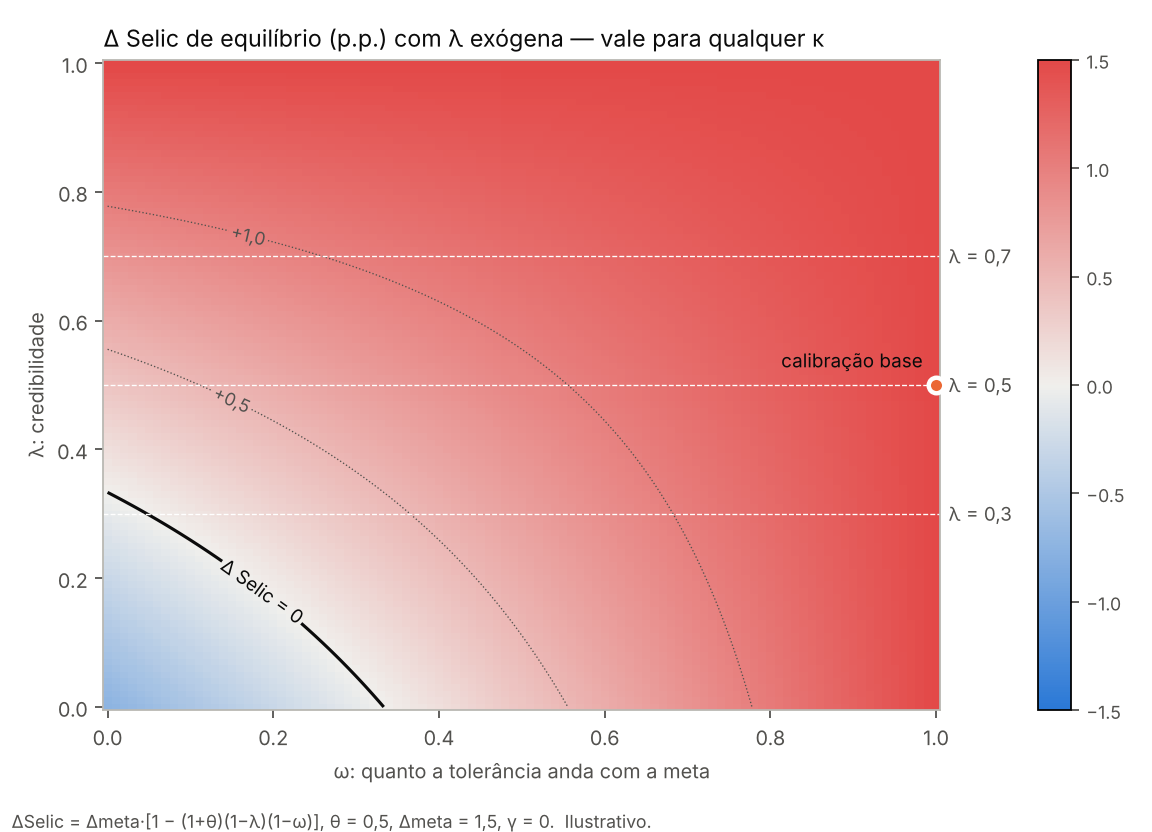
\includegraphics[width=0.75\textwidth]{mapa_lambda_exogena.png}
\caption{Credibilidade exógena: variação da Selic de equilíbrio (p.p.) ao subir a meta de 3\% para 4,5\%, em função de $\omega$ e $\lambda$ ($\gamma=0$). O resultado vale para qualquer $\kappa$.}
\label{fig:mapa_exo}
\end{figure}

\subsection{Estimação com dados do Brasil}

\paragraph{Dados.}
\begin{itemize}
  \item \textbf{Expectativas de mercado (Focus/BCB):} medianas das projeções de IPCA para os anos-calendário $t+1$ a $t+4$ e para os próximos 12 meses (série suavizada), de dezembro de 2001 a novembro de 2026. Agregamos as observações diárias pela média mensal.
  \item \textbf{Metas do CMN:} reconstruímos, para cada mês, a meta \emph{conhecida} para cada ano de referência, a partir das datas dos anúncios. Quando a meta de um ano ainda não havia sido anunciada, usamos a última meta anunciada, que é a melhor previsão do mercado. Incluímos as metas ajustadas de janeiro de 2003 e a meta contínua de 3\% a partir de junho de 2023.
  \item \textbf{IPCA acumulado em 12 meses} (SGS 13522), usado como referência.
\end{itemize}

\paragraph{Horizonte constante.} As projeções do Focus são por ano-calendário: a projeção para ``$t+3$'' feita em janeiro cobre um horizonte de 36 meses, mas a feita em dezembro cobre 25 meses, e em todo janeiro o ano de referência muda. Isso gera saltos que não refletem mudança de expectativa. Seguindo procedimento já usado pelo BCB, construímos a expectativa para os 12 meses que terminam em $t+36$ interpolando os anos-calendário pelos meses que cada um contribui. No mês $m$ do ano $Y$, esse período cobre $12-m$ meses de $Y+2$ e $m$ meses de $Y+3$:
\begin{equation}
\pe_t(36) = \frac{12-m}{12}\,\pe_t(Y+2) + \frac{m}{12}\,\pe_t(Y+3) .
\end{equation}
A meta de mesmo horizonte é interpolada da mesma forma. Para o curto prazo, usamos a expectativa do Focus para os 12 meses seguintes, que já tem horizonte constante. Usamos 36 meses como horizonte principal porque ele está além da defasagem da política monetária: a expectativa nesse prazo reflete a crença sobre a meta, não sobre choques correntes.

\paragraph{Frequência trimestral.} Agregamos as séries mensais pela média do trimestre (2002T1 a 2026T4, com o último trimestre parcial). A agregação reduz o ruído das medianas do Focus, que tendem a ficar paradas em números redondos e a mudar em saltos.

\paragraph{Desancoragem.} É a diferença entre a expectativa e a meta no horizonte de 36 meses, $\pe(36)-\meta(36)$.

\paragraph{Credibilidade $\lambda$.} Se as expectativas estão ancoradas, revisões das projeções de curto prazo não contaminam as de longo prazo. Estimamos, em janelas móveis de 16 trimestres,
\begin{equation}
\Delta\pe_{q}(36) = c + \beta\,\Delta\pe_{q}(12) + \varepsilon_q, \qquad \lambda_q = 1-\beta_q ,
\end{equation}
limitando $\lambda_q$ ao intervalo $[0,1]$.

\paragraph{Leniência $\kappa$.} Da identidade do modelo, $\pe-\meta=(1-\lambda)\kappa$, logo $\kappa=(\pe-\meta)/(1-\lambda)$.

\paragraph{Repasse e $\omega$: estudo de evento.} Para cada anúncio do CMN que mudou a meta de um ano, medimos a variação da expectativa para \emph{aquele ano} entre o mês anterior ao anúncio e dezembro do mesmo ano. Aqui usamos o ano-calendário, e não o horizonte constante, porque o anúncio muda a meta de um ano específico. Em 2017, usamos fevereiro como mês pré, porque a redução já era discutida antes do anúncio. O repasse é $b = \Delta\pe / \dmeta$. Pelas equações (1) e (2), com $\gamma=0$, o repasse teórico é
\begin{equation}
b = \lambda + (1-\lambda)\,\omega \quad\Longrightarrow\quad \omega = \frac{b-\lambda}{1-\lambda},
\end{equation}
com $\lambda$ medido no trimestre anterior a cada anúncio.

\paragraph{Resultados.} A Figura~\ref{fig:estim_exo} resume os dados. Nas seis mudanças de meta entre 2017 e 2021, o repasse foi praticamente um para um (média de 0,98). Com $\lambda$ médio de 0,70 antes dos eventos, obtemos $\omega = 0{,}94$: a tolerância percebida acompanha a meta quase integralmente. A credibilidade estimada caiu de valores próximos de 1 em 2020--2022 para 0,74 em 2026.

\begin{figure}[H]
\centering
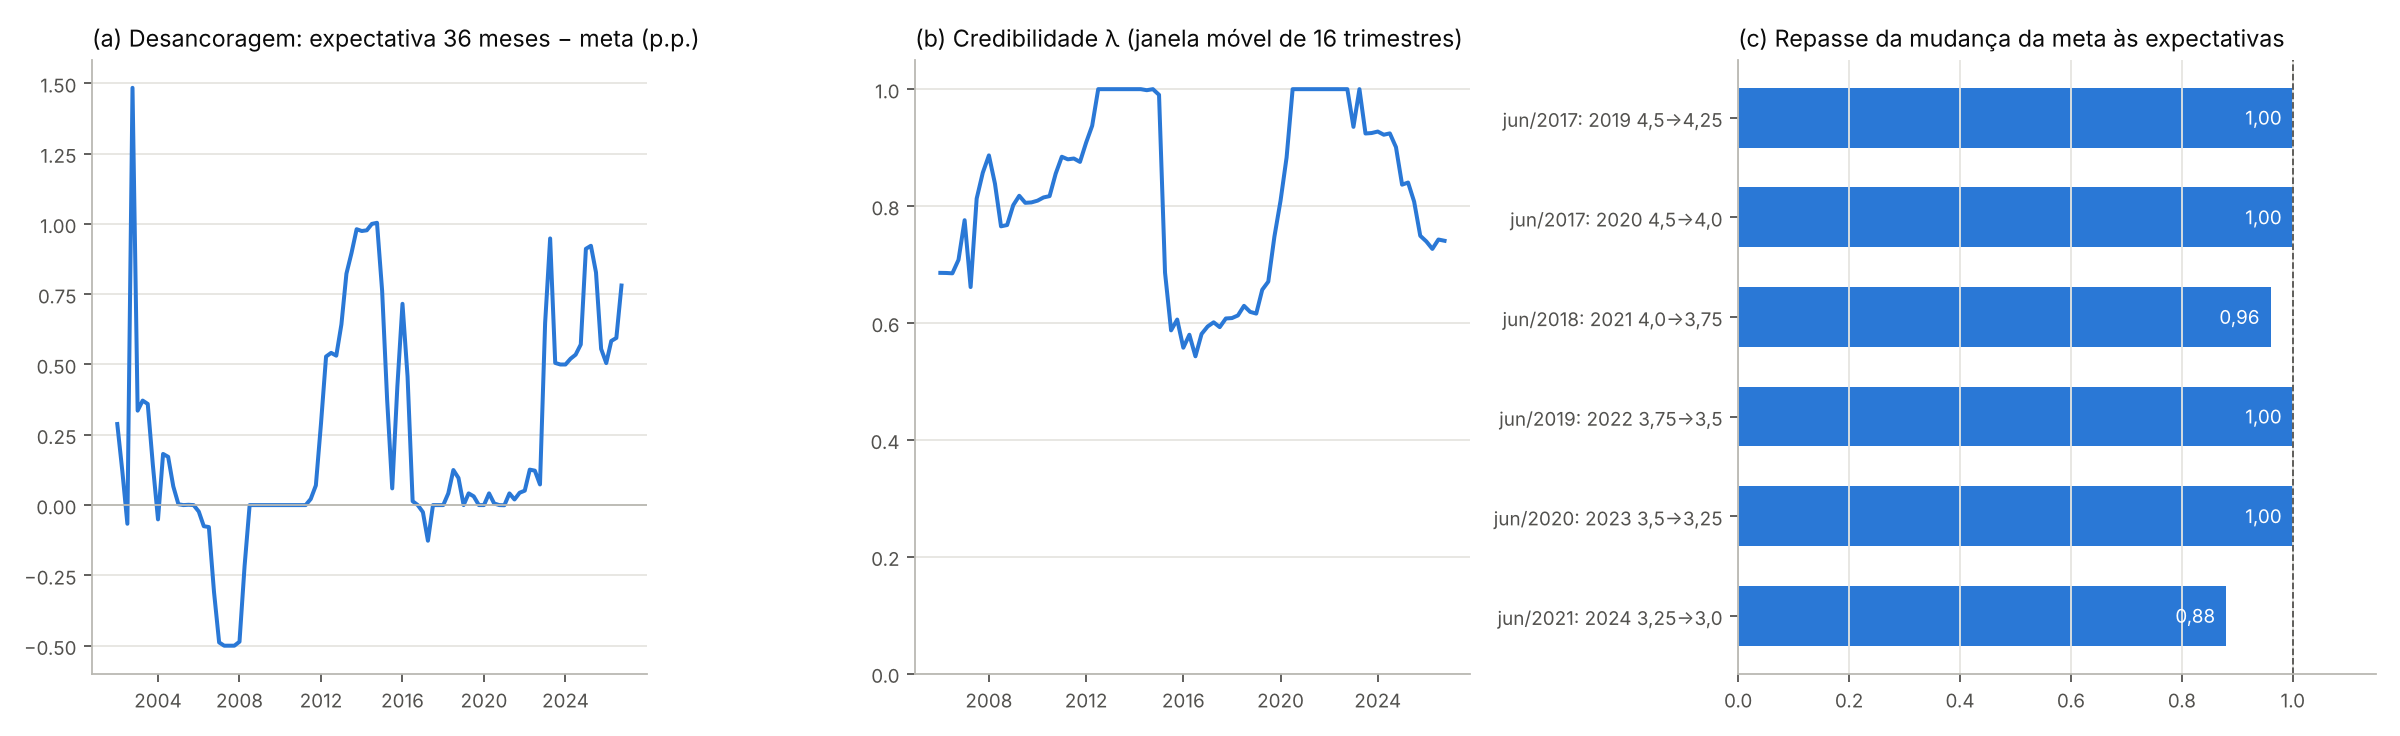
\includegraphics[width=\textwidth]{fig_estim_exogena.png}
\caption{(a) Desancoragem no horizonte de 36 meses; (b) credibilidade $\lambda$ estimada em janelas de 16 trimestres; (c) repasse das mudanças de meta às expectativas do ano afetado. Fontes: BCB/Focus, SGS, CMN.}
\label{fig:estim_exo}
\end{figure}

\begin{table}[H]
\centering
\begin{tabular}{lcccc}
\toprule
Evento & $\dmeta$ & $\Delta\pe$ & Repasse & $\lambda$ pré \\
\midrule
jun/2017: 2019, 4,5 $\to$ 4,25 & $-0{,}25$ & $-0{,}25$ & 1,00 & 0,58 \\
jun/2017: 2020, 4,5 $\to$ 4,0 & $-0{,}50$ & $-0{,}50$ & 1,00 & 0,58 \\
jun/2018: 2021, 4,0 $\to$ 3,75 & $-0{,}25$ & $-0{,}24$ & 0,96 & 0,61 \\
jun/2019: 2022, 3,75 $\to$ 3,5 & $-0{,}25$ & $-0{,}25$ & 1,00 & 0,62 \\
jun/2020: 2023, 3,5 $\to$ 3,25 & $-0{,}25$ & $-0{,}25$ & 1,00 & 0,81 \\
jun/2021: 2024, 3,25 $\to$ 3,0 & $-0{,}25$ & $-0{,}22$ & 0,88 & 1,00 \\
\midrule
\multicolumn{3}{l}{Repasse médio (MQO pela origem)} & 0,98 & 0,70 \\
\bottomrule
\end{tabular}
\caption{Estudo de evento das mudanças de meta do CMN.}
\end{table}

Um ponto chama atenção: em 2017--2019 a credibilidade estimada estava entre 0,6 e 0,8, e mesmo assim o repasse foi completo. Pelo modelo, isso só é possível se a parte não ancorada das expectativas também acompanha a meta, ou seja, $\omega$ próximo de 1.

\paragraph{Simulação com os parâmetros estimados.} Partimos do 3º trimestre de 2026, o último completo: desancoragem de 0,59 p.p. e $\lambda=0{,}74$, o que implica $\kappa=2{,}3$. Mantemos $\theta=0{,}5$ e $r^{*}=5\%$, que não foram estimados.

\begin{table}[H]
\centering
\begin{tabular}{lcccc}
\toprule
 & \multicolumn{3}{c}{$\gamma$} \\
\cmidrule(lr){2-4}
 & 0 & 0,05 & 0,10 \\
\midrule
$\omega$ estimado (0,94) & $+1{,}47$ & $+1{,}72$ & $+1{,}97$ \\
$\omega = 0$ (teto fixo) & $+0{,}92$ & $+1{,}01$ & $+1{,}10$ \\
\bottomrule
\end{tabular}
\caption{Credibilidade exógena, parâmetros estimados: variação da Selic de equilíbrio (p.p.) ao subir a meta de 3\% para 4,5\%. Base: 3º trimestre de 2026. Valores de $\gamma$ simulados; a calibração está na Seção~\ref{sec:gamma}.}
\label{tab:res_exo}
\end{table}

Mesmo o caso de teto fixo ($\omega=0$) fica longe da região em que a Selic cai: com $\theta=0{,}5$, a condição $(1-\lambda)(1-\omega) > 2/3$ exigiria $\lambda < 1/3$, menos da metade da credibilidade estimada hoje.

%=====================================================================
\section{Parte II: credibilidade endógena}

\subsection{O modelo}

Se as expectativas já estão desancoradas, a credibilidade já é baixa. Substituímos a equação (3) por
\begin{equation}
\lambda = \bar\lambda - \eta\,(\pe - \meta) - \gamma\,\dmeta ,
\end{equation}
em que $\bar\lambda$ é a credibilidade máxima, com expectativas perfeitamente ancoradas, e $\eta$ mede quanto a desancoragem corrói a credibilidade. As demais equações não mudam.

\subsection{Solução}

Combinando com $\pe-\meta=(1-\lambda)K$:
\begin{equation}
\boxed{\;\pe - \meta = \frac{(1-\bar\lambda+\gamma\,\dmeta)\,K}{1-\eta K}\;}
\end{equation}
O termo $1/(1-\eta K)$ é um \textbf{multiplicador}: a desancoragem reduz a credibilidade, que aumenta a desancoragem. Se $\eta K \geq 1$, o multiplicador explode: a credibilidade vai a zero e as expectativas perdem a âncora (ponto de não retorno).

O mecanismo corta nos dois sentidos:
\begin{itemize}
  \item Com $\gamma>0$, a perda de credibilidade causada pela mudança é amplificada.
  \item Com $\omega<1$, subir a meta reduz $K$ de forma mecânica. A desancoragem cai, a credibilidade melhora, e o multiplicador amplifica a melhora. É aqui que aparece o cenário em que subir a meta ajuda.
\end{itemize}

\subsection{Sensibilidades}

A Figura~\ref{fig:mapa_endo} usa uma calibração estilizada: $\bar\lambda=0{,}8$, $\eta=0{,}2$ e $\kappa=3$, que reproduz expectativas em 4,5\% com meta de 3\% e $\lambda=0{,}5$ (multiplicador de 2,5).

\begin{figure}[H]
\centering
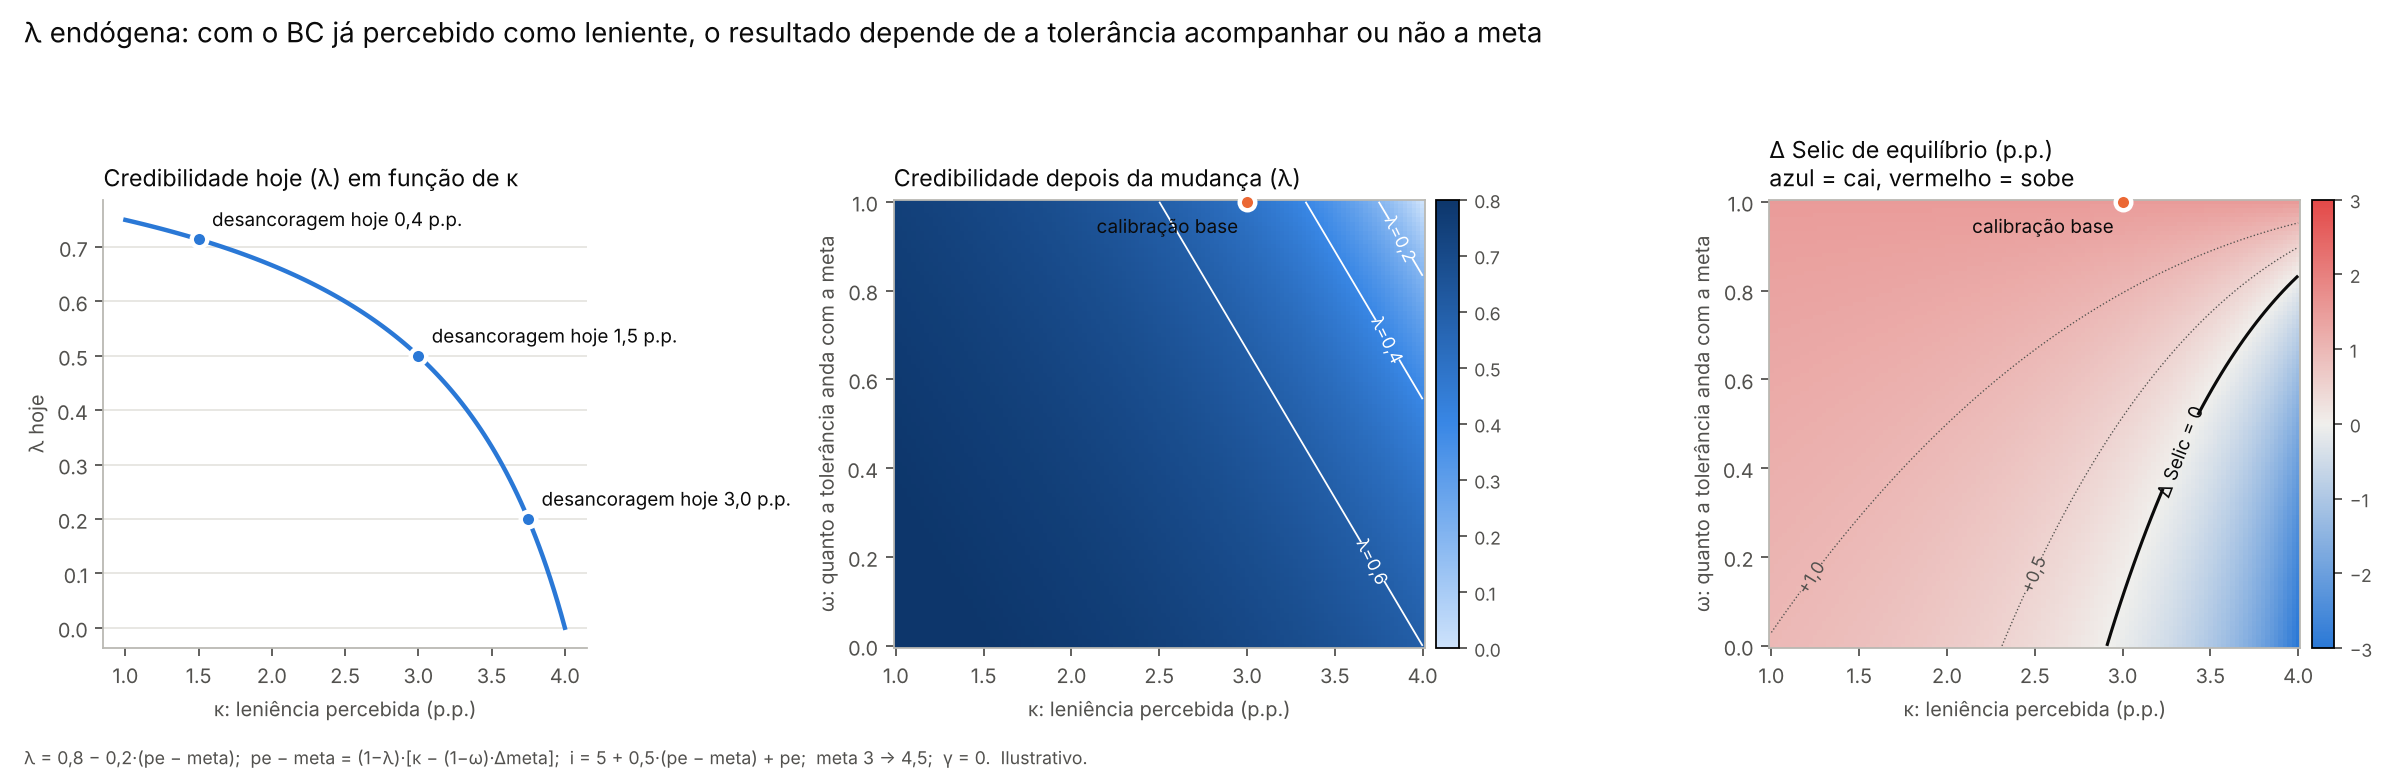
\includegraphics[width=\textwidth]{mapa_lambda_endogena.png}
\caption{Credibilidade endógena ($\gamma=0$). Esquerda: credibilidade atual em função da leniência $\kappa$. Centro: credibilidade depois da mudança. Direita: variação da Selic de equilíbrio (p.p.); a linha preta marca $\Delta i = 0$.}
\label{fig:mapa_endo}
\end{figure}

A Figura~\ref{fig:mapa_endo} mostra que a região em que a Selic cai é maior que no caso exógeno: com leniência alta ($\kappa$ próximo do ponto de não retorno) e tolerância fixa ($\omega=0$), a queda pode chegar a 1,8 p.p. É o cenário ``a meta atual é irrealista, e alinhá-la reancora as expectativas''. Esse cenário exige três condições ao mesmo tempo: credibilidade já muito baixa, expectativas presas a um nível que não depende da meta, e nenhuma perda de credibilidade com a mudança ($\gamma\approx 0$).

\subsection{Estimação com dados do Brasil}

\paragraph{Metodologia.} Usamos as mesmas séries trimestrais da Parte I. A equação de credibilidade é estimada por MQO:
\begin{equation}
\lambda_q = \bar\lambda - \eta\,\overline{(\pe-\meta)}_{q-4} + u_q ,
\end{equation}
em que $\lambda_q$ é a credibilidade estimada em janelas de 16 trimestres e $\overline{(\pe-\meta)}_{q-4}$ é a desancoragem média dos 16 trimestres anteriores, defasada 4 trimestres para reduzir a simultaneidade. Como as janelas móveis geram autocorrelação forte nos resíduos, os erros-padrão são de Newey-West com 8 defasagens. A amostra vai até o 3º trimestre de 2026. O parâmetro $\kappa$ é obtido do ponto fixo do modelo, de modo a reproduzir a desancoragem observada:
\begin{equation}
\kappa = \frac{(\pe-\meta)_0}{(1-\bar\lambda) + \eta\,(\pe-\meta)_0} .
\end{equation}
$\omega$ vem do estudo de evento da Parte I.

\paragraph{Resultados.} Estimamos $\bar\lambda = 0{,}89$ (EP 0,04) e $\eta = 0{,}37$ (EP 0,10), com 80 observações trimestrais. O sinal é o esperado e o coeficiente é significativo (estatística $t$ de 3,6): cada ponto percentual de desancoragem nos quatro anos anteriores reduz a credibilidade em cerca de 0,37. A equação reproduz bem os grandes movimentos de $\lambda$, como a queda em 2015--2016 e a recuperação depois de 2018 (Figura~\ref{fig:estim_endo}).

\begin{figure}[H]
\centering
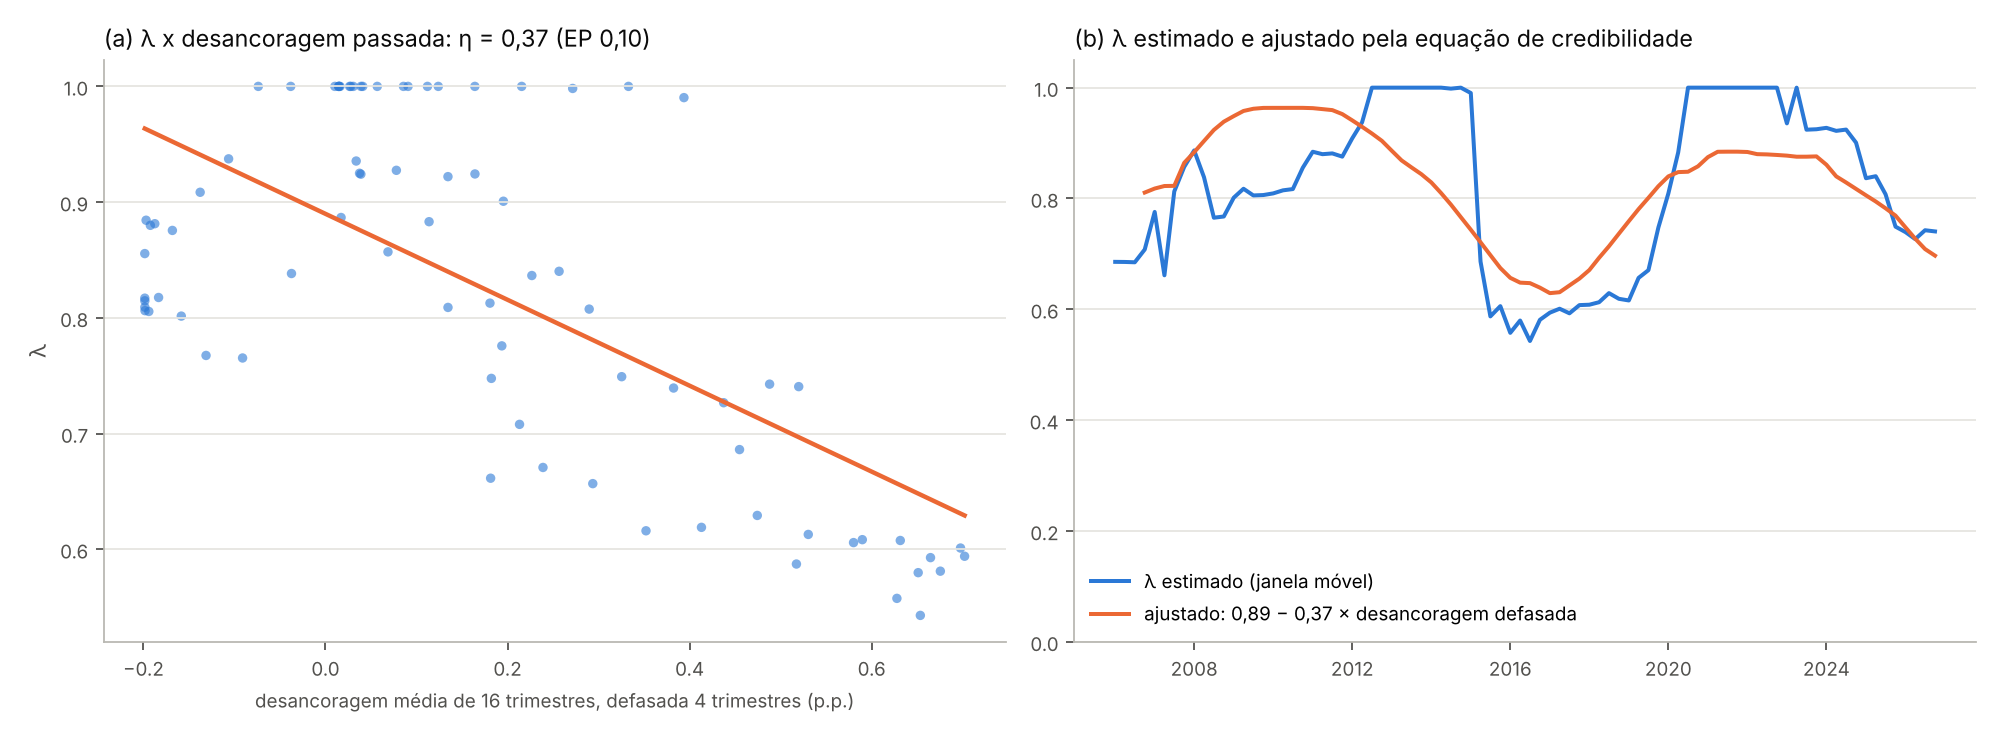
\includegraphics[width=\textwidth]{fig_estim_endogena.png}
\caption{(a) Credibilidade estimada contra a desancoragem passada e reta ajustada; (b) credibilidade estimada e ajustada pela equação de credibilidade.}
\label{fig:estim_endo}
\end{figure}

Com a desancoragem do 3º trimestre de 2026 (0,59 p.p.), obtemos $\kappa=1{,}8$, $\lambda=0{,}67$ e multiplicador $1/(1-\eta\kappa)$ de 3,0: a desancoragem atual é três vezes a que existiria sem o círculo vicioso entre desancoragem e credibilidade.

\begin{table}[H]
\centering
\begin{tabular}{lcccc}
\toprule
 & \multicolumn{3}{c}{$\gamma$} \\
\cmidrule(lr){2-4}
 & 0 & 0,05 & 0,10 \\
\midrule
$\omega$ estimado (0,94) & $+1{,}38$ & $+1{,}90$ & $+2{,}43$ \\
$\omega = 0$ (teto fixo) & $+0{,}66$ & $+0{,}70$ & $+0{,}74$ \\
\bottomrule
\end{tabular}
\caption{Credibilidade endógena, parâmetros estimados: variação da Selic de equilíbrio (p.p.) ao subir a meta de 3\% para 4,5\%. Base: 3º trimestre de 2026. Valores de $\gamma$ simulados; a calibração está na Seção~\ref{sec:gamma}.}
\label{tab:res_endo}
\end{table}

Com o $\omega$ estimado, o multiplicador amplifica a perda de credibilidade: com $\gamma=0{,}10$, $\lambda$ cai de 0,67 para 0,29 e a Selic sobe 2,4 p.p. No caso mais favorável à mudança ($\omega=0$, $\gamma=0$), a credibilidade melhora, mas a Selic ainda sobe cerca de 0,7 p.p. A região em que ela cai, que existe na teoria, fica longe dos parâmetros estimados para o Brasil.

%=====================================================================
%=====================================================================
\section{Dois episódios do histórico}

\paragraph{2023: o custo de discutir a meta.} No horizonte de 36 meses, a desancoragem passou de 0,07 p.p. no 4º trimestre de 2022 para 0,95 p.p. no 2º trimestre de 2023, sem nenhuma mudança na meta, e ficou em 0,5 p.p. depois que o CMN manteve os 3\%. A Seção~\ref{sec:gamma} usa esse episódio para estimar $\gamma$.

\paragraph{Janeiro de 2003: o único aumento de meta.} A meta de 2004 subiu de 3,75\% para 5,5\%, com desancoragem inicial de 3,8 p.p. A expectativa para 2004 caiu 0,2 p.p., padrão compatível com o cenário de teto fixo e credibilidade baixa. O episódio, porém, coincide com a troca de comando do BC e com a elevação da Selic a 26,5\%. Não é possível atribuir o efeito à meta, e a Selic, de todo modo, subiu.

%=====================================================================
\section{Impacto estimado de uma mudança da meta hoje}

Juntamos as estimativas para responder à pergunta prática: o que aconteceria se a meta fosse elevada de 3\% para 4,5\% a partir da situação atual? Usamos a versão com credibilidade endógena, porque a relação entre desancoragem e credibilidade é estatisticamente significativa nos dados, e o $\omega$ estimado (0,94). O ponto de partida é o 3º trimestre de 2026: expectativa em 36 meses de 3,59\%, desancoragem de 0,59 p.p., credibilidade de 0,67 e Selic neutra nominal de 8,9\% no modelo ($r^{*}=5\%$). Nas Partes I e II, a perda de credibilidade causada pela mudança, $\gamma$, foi tratada com valores simulados. Aqui, primeiro a calibramos com o episódio de 2023 e depois calculamos o impacto.


\subsection{Calibrando a perda de credibilidade $\gamma$: o episódio de 2023}
\label{sec:gamma}

O parâmetro $\gamma$ mede quanta credibilidade se perde quando a meta \emph{sobe}. No Brasil, a meta só subiu uma vez na amostra, em janeiro de 2003, num episódio contaminado pela troca de comando do BC. Não há, portanto, como estimar $\gamma$ diretamente. O debate de 2023 oferece uma alternativa: houve uma ameaça crível de mudança, com tamanho definido, e depois a mudança foi descartada. Em 18 de janeiro de 2023, o presidente da República afirmou que a meta ideal para o Brasil seria de 4,5\%, exatamente a mudança de 3\% para 4,5\% que simulamos. O debate se estendeu até 29 de junho, quando o CMN manteve a meta de 3\% e adotou a meta contínua.

\begin{figure}[H]
\centering
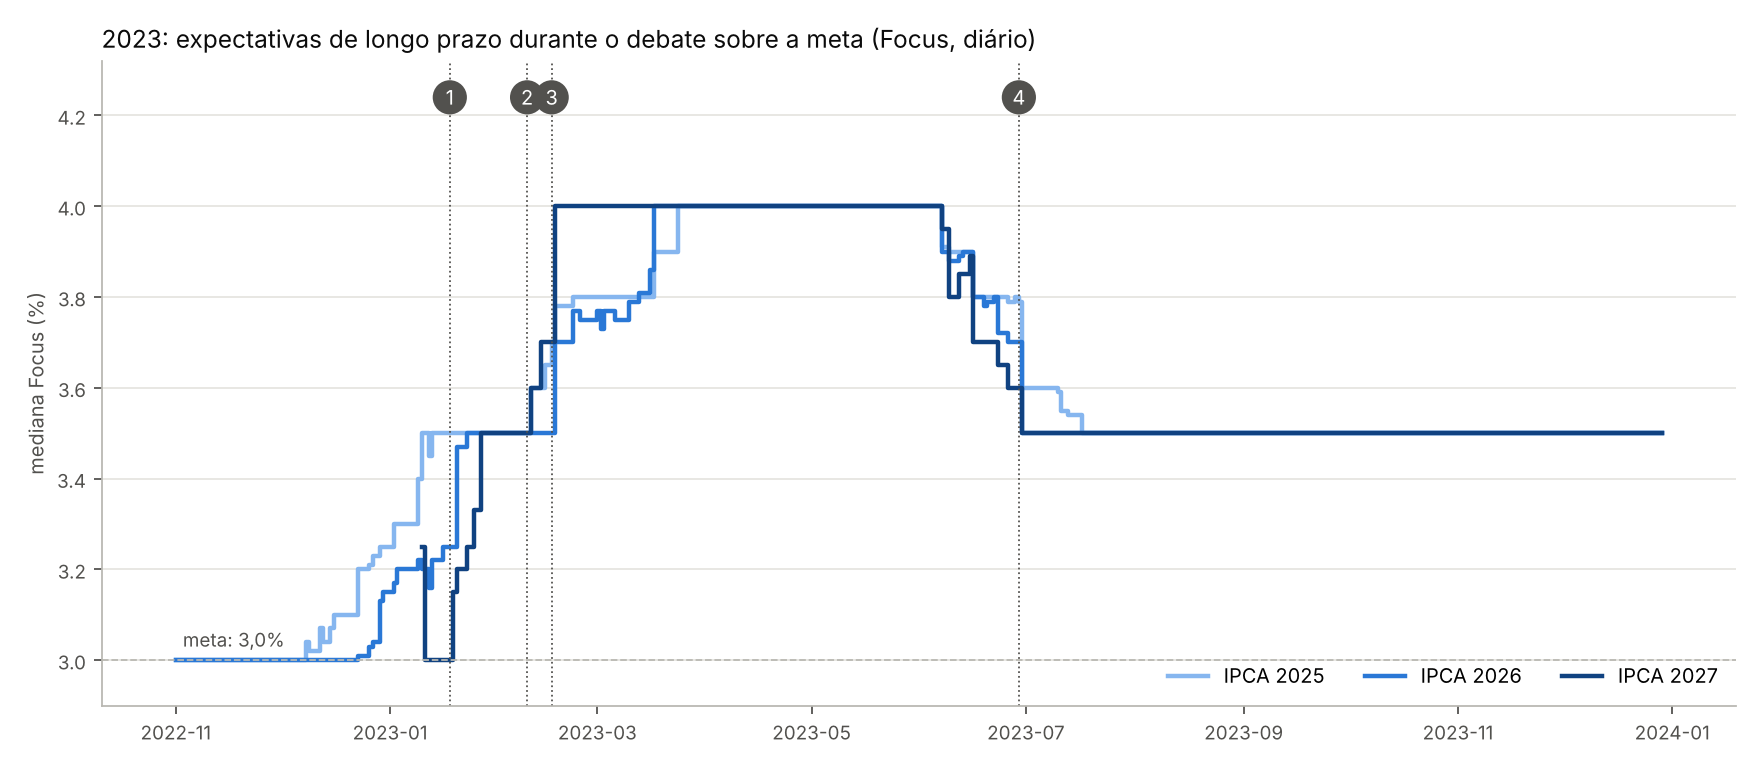
\includegraphics[width=\textwidth]{fig_2023.png}
\caption{Medianas diárias do Focus para o IPCA de 2025, 2026 e 2027. (1) 18/01: o presidente defende meta de 4,5\%; (2) 09/02: notícia de que o governo estudava antecipar o debate; (3) 16/02: reunião do CMN; (4) 29/06: CMN mantém a meta de 3\% e adota a meta contínua. A projeção para 2027 passa a ser coletada em janeiro de 2023.}
\label{fig:2023}
\end{figure}

\paragraph{Identificação.} Seja $p$ a probabilidade que o mercado atribuía à mudança de tamanho $D=1{,}5$ p.p., e $E$ a desancoragem adicional causada pela perda de credibilidade. Com repasse $b$ estimado no estudo de evento:
\begin{align}
\text{pico} - \text{base} &= p\,D\,b + E, \\
\text{queda com a decisão de manter a meta} &= p\,D\,b, \\
\text{pós} - \text{base} &= E.
\end{align}
A segunda equação supõe que a perda de credibilidade não se reverte quando a meta é mantida. A desancoragem adicional por ponto percentual de mudança esperada é $e = E/(p\,D)$. Escolhemos $\gamma$ de modo que o modelo com credibilidade endógena e os parâmetros estimados na Seção~3, partindo do 3º trimestre de 2026, gere a mesma desancoragem adicional por ponto percentual de mudança efetiva da meta.

\paragraph{Resultados.} As expectativas para 2026 e 2027 subiram até 4,0\%, caíram 0,5 p.p. entre os sinais de junho e a decisão do CMN e ficaram estáveis em 3,5\% até o fim do ano (Figura~\ref{fig:2023}). A queda implica que o mercado atribuía cerca de um terço de probabilidade à mudança.

\begin{table}[H]
\centering
\begin{tabular}{lcccccc}
\toprule
Série e base & Subida & Queda & $p$ & $E$ & $e$ & $\gamma$ \\
\midrule
IPCA 2026, base 18/01/2023 & 0,75 & 0,50 & 0,34 & 0,25 & 0,49 & 0,10 \\
IPCA 2026, base dez/2022 & 1,00 & 0,50 & 0,34 & 0,50 & 0,98 & 0,17 \\
IPCA 2027, base 18/01/2023 & 1,00 & 0,50 & 0,34 & 0,50 & 0,98 & 0,17 \\
\bottomrule
\end{tabular}
\caption{Calibração de $\gamma$ pelo episódio de 2023. Subida, queda e $E$ em p.p.; $e$ é a desancoragem adicional por p.p. de mudança esperada da meta.}
\label{tab:gamma}
\end{table}

A estimativa mais conservadora, $\gamma=0{,}10$, usa a série de 2026 com base no dia da entrevista, o que exclui a alta de dezembro e início de janeiro associada à transição fiscal. As demais incluem toda a alta e chegam a $\gamma=0{,}17$, valor em que a credibilidade do modelo vai a zero. Os dois valores ficam acima da faixa de 0 a 0,10 usada como simulação nas Partes I e II.

\paragraph{Ressalvas.} Dois vieses operam em sentidos opostos. Em 2023, a mudança fiscal e as críticas à autonomia do BC também pesaram sobre as expectativas, o que tende a superestimar $\gamma$. Já a decisão de junho também trouxe a meta contínua, que pode ter recuperado credibilidade por conta própria; nesse caso, parte da queda não reflete o fim da ameaça, $p$ está superestimado e $\gamma$, subestimado. A base no dia da entrevista atenua o primeiro viés.

\subsection{Impacto estimado}

Para a perda de credibilidade causada pela própria mudança, usamos as estimativas da Seção~\ref{sec:gamma}: $\gamma=0{,}10$ como cenário central, por ser a estimativa mais conservadora, e $\gamma=0{,}17$ como cenário pessimista. O cenário otimista supõe $\gamma=0$, isto é, nenhuma perda de credibilidade.

\begin{table}[H]
\centering
\begin{tabular}{lccccc}
\toprule
Cenário & $\pe(36)$ & Desancoragem & $\lambda$ & Selic neutra & $\Delta$ Selic \\
\midrule
Hoje (meta de 3\%) & 3,59 & 0,59 & 0,67 & 8,9 & -- \\
\midrule
Otimista ($\gamma=0$) & 5,01 & 0,51 & 0,70 & 10,3 & $+1{,}4$ \\
\textbf{Central ($\gamma=0{,}10$)} & \textbf{5,75} & \textbf{1,25} & \textbf{0,27} & \textbf{11,4} & $\mathbf{+2{,}5}$ \\
Pessimista ($\gamma=0{,}17$) & 6,21 & 1,71 & 0,00 & 12,1 & $+3{,}2$ \\
\midrule
\emph{Teto fixo ($\omega=0$, $\gamma=0$), não corroborado} & 4,54 & 0,04 & 0,88 & 9,6 & $+0{,}7$ \\
\bottomrule
\end{tabular}
\caption{Impacto estimado de elevar a meta de 3\% para 4,5\%, partindo do 3º trimestre de 2026. Credibilidade endógena, $\omega=0{,}94$. Expectativa, desancoragem e Selic em \% ou p.p.; a desancoragem é medida em relação à nova meta.}
\label{tab:impacto}
\end{table}

No cenário central:
\begin{itemize}
  \item A expectativa de inflação em 36 meses sobe de 3,6\% para 5,75\%, ou seja, 2,2 p.p., \emph{mais} do que a mudança da meta.
  \item A desancoragem não desaparece: passa de 0,59 p.p. em relação à meta de 3\% para 1,25 p.p. em relação à nova meta de 4,5\%.
  \item A credibilidade cai de 0,67 para 0,27, e o multiplicador amplifica essa perda.
  \item A Selic neutra nominal sobe de 8,9\% para 11,4\%, cerca de 2,5 p.p. O juro real neutro também sobe, pelo prêmio de risco associado à desancoragem maior.
\end{itemize}

Mesmo no cenário otimista, sem nenhuma perda de credibilidade, a Selic neutra sobe 1,4 p.p. A única configuração que reduz o aumento para menos de 1 p.p. é a de teto fixo, que o estudo de evento rejeita. Partindo do 4º trimestre de 2026, ainda parcial e com desancoragem maior (0,78 p.p.), o cenário central indica alta de 2,8 p.p.

%=====================================================================
\section{Conclusão}

Existe um cenário em que subir a meta ajuda a Selic a cair. Ele exige credibilidade muito baixa, expectativas presas a um nível que não depende da meta, nenhuma perda de credibilidade com a mudança e, no caso de credibilidade exógena, um prêmio de risco que caia só porque a régua foi redefinida.

O histórico brasileiro não corrobora esse cenário; pelo contrário:
\begin{enumerate}
  \item As expectativas acompanharam as mudanças de meta quase um para um entre 2017 e 2021 ($\omega=0{,}94$), mesmo em períodos de credibilidade moderada. A tolerância percebida anda com a meta.
  \item A desancoragem passada reduz a credibilidade de forma significativa ($\eta=0{,}37$). Com o multiplicador atual de 3,0, qualquer perda de credibilidade causada pela mudança é amplificada.
  \item A discussão sobre mudar a meta, em 2023, desancorou as expectativas sem que nada tivesse mudado. Calibrado por esse episódio, o custo de credibilidade de uma mudança efetiva ($\gamma$ entre 0,10 e 0,17) é alto.
\end{enumerate}

Com os parâmetros estimados, elevar hoje a meta de 3\% para 4,5\% levaria a expectativa de inflação em 36 meses para cerca de 5,75\% e aumentaria a Selic neutra nominal em cerca de 2,5 p.p., de 8,9\% para 11,4\%, no cenário central. O intervalo vai de 1,4 a 3,2 p.p., conforme a perda de credibilidade suposta. O resultado mais provável não é juro menor, mas inflação e juro nominal maiores, com credibilidade menor.

%=====================================================================
\section{Limitações}

\begin{itemize}
  \item O modelo é de estado estacionário e não captura a dinâmica de transição.
  \item $\theta$ e $r^{*}$ foram calibrados, não estimados.
  \item Mesmo com dados trimestrais, as medianas do Focus de longo prazo ficam paradas em números redondos, o que pode superestimar $\lambda$ em alguns períodos (valores iguais a 1).
  \item $\gamma$ é calibrado por um único episódio, de ameaça e não de mudança efetiva, e supõe que a perda de credibilidade não se reverteu quando a meta foi mantida.
  \item $\omega$ vem de seis eventos, todos de \emph{redução} da meta. Um aumento pode ter efeito assimétrico, provavelmente com $\gamma$ maior.
  \item A interpolação para horizonte constante supõe que a inflação esperada se distribui de forma uniforme dentro de cada ano-calendário.
  \item O 4º trimestre de 2026 é parcial e mostra desancoragem de 0,78 p.p. Com esse ponto de partida, as conclusões se mantêm.
\end{itemize}

\vspace{1em}
{\footnotesize\color{gray} Fontes: Banco Central do Brasil (Sistema de Expectativas de Mercado -- Focus; SGS série 13522) e resoluções do Conselho Monetário Nacional. Modelo ilustrativo; os números mostram o mecanismo e não são projeções.}

\end{document}
